\documentclass{standalone}
\usepackage{tikz}
\begin{document}
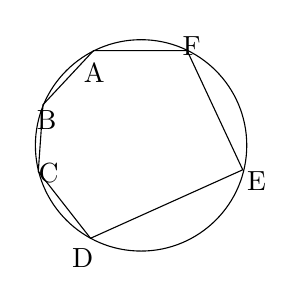
\begin{tikzpicture}[x=1pt,y=1pt]
\draw (147.41,-161.46) circle (38.19);
\node at (130.49,-135.47) {A};
\node at (113.31,-152.30) {B};
\node at (114.00,-171.53) {C};
\node at (126.34,-202.31) {D};
\node at (189.12,-174.51) {E};
\node at (165.70,-125.68) {F};
\draw (164.05,-127.20) -- (130.24,-127.20) -- (111.97,-146.76) -- (110.27,-170.89) -- (129.15,-195.03) -- (184.15,-170.28) -- cycle;
\end{tikzpicture}
\end{document}
